% !TEX root = ../main.tex

\chapter{Creativity}
\label{ch:creativity}

\startcontents[chapters]

\vfill

\begin{alltt}\sffamily
From high Olympus prone her flight she bends,
rare courage and grandeur of conception,
congratulating herself apparently on the cleverness with which she had managed her expedition,
appeared distorted to my vision.

Had he had any bad design,
having uttered these words the vision left me,
if any thought by flight to escape,
taking his flight towards warmer and sunnier regions.

Inspire à mon oncle cette vision décourageante de l'avenir,
être et l'invention du jeu de ce,
besoin de satisfaire l'imagination d'objets rares ou grandioses.

Some may call vision,
a man of invaluable ability,
mobiles parois de L'imagination.
\end{alltt}

\newpage
\minicontents
\spirals

Creativity does not have a universally accepted definition. Creativity is a human quality and definitions don't necessarily lend themselves to be applied to computers as well. There are aspects that come up in many, like novelty and value, but some that rarely pop up, like relevance and variety. Creativity can be studied at various `levels' (neurological, cognitive, and holistic/systemic), from different `perspectives' (subjective and objective) and `characteristics' (combinational, exploratory and transformative). Creativity should be seen as a continuum, there is no clear cut-off point or Boolean answer to say precisely when a person or piece of software has become creative or not.

Linda Candy identified 3 approaches for studying creativity \citeyear[p.3]{Candy2012}:

\begin{description}
  \item [Research Design] Experimental, psychometric, observational, \ldots
  \item [Research Focus] Human attributes, cognitive processes or creative outcomes.
  \item [Research Evidence] Real-time observation, historical data, artificial (laboratory) or natural (real world settings).
\end{description}

Richard Mayer identified five big questions of human creativity research and different approaches with their own methodologies and goals \citeyear[p.450-451,453]{Mayer1999}:

\label{s:Mayer5questions}
\begin{enumerate}
  \item Is creativity a property of people, products, or processes?
  \item Is creativity a personal or social phenomenon?
  \item Is creativity common or rare?
  \item Is creativity domain-general or domain-specific?
  \item Is creativity quantitative or qualitative?
\end{enumerate}

\begin{description}
  \item [Psychometric] (creativity as a mental trait): quantitative measurement, controlled environments, ability based analysis
  \item [Psychological] (creativity as cognitive processing): controlled environments, quantitative measurements, cognitive task analysis
  \item [Biographical] (creativity as a life story): authentic environments, qualitative descriptions, quantitative measurements
  \item [Biological] (creativity as a physiological trait): physiological measures
  \item [Computational] (creativity as a mental computation): formal modelling
  \item [Contextual] (creativity as a context-based activity): social, cultural and evolutionary context
\end{description}

Mayer identified the challenge of developing a ``clearer definition of creativity'' and ``a combination of research methodologies that will move the field from speculation to specification'' \citeyear[p.459]{Mayer1999} which are addressed in chapter~\ref{ch:methodology}\marginnote{§~\ref{ch:methodology}}.

This chapter introduces relevant models of human and computer creativity and describes the disciplines of computational creativity and creative computing.


\section{In Humans}
\label{s:humancreativity}

Let us define creativity as \emph{the ability to use original ideas to create something new and surprising of value}. We generally speak of creative ideas rather than products, since creative products merely provide evidence of a creative process that has already taken place.

\begin{quotation}
  Creativity is the interaction among aptitude, process, and environment by which an individual or group produces a perceptible product that is both novel and useful as defined within a social context \sourceatright{\autocite[Plucker et al in][p.90]{Jordanous2012}}
\end{quotation}


\subsection{Four Stages}
\label{s:4stages}

Henri Poincar{\'e} and Graham Wallas have defined a popular model of the creative process (it was suggested by Poincar{\'e} \citeyear[p.387--400]{Poincare2001} and formulated by Wallas \citeyear{Wallas1926}). This model has been picked up by many researchers since, including \autocite{Boden2003, Koestler1964, Partridge1994}.

\begin{enumerate}
  \item Preparation – focusing the mind on the problem
  \item Incubation – unconscious internalising
  \item Illumination – eureka moment from unconsciousness to consciousness
  \item Verification – conscious evaluation of the idea and elaboration…
\end{enumerate}

Weisberg, however, criticises the stages of incubation and illumination \autocite[as cited in][]{Partridge1994}, saying that the creative process is really just simple problem solving, and that incubation is what he calls `creative worrying'. Problem solving was defined in similar steps by George Polya in 1957 \citeyear{Polya1957}.

\begin{quotation}
  First, we have to \textbf{understand} the problem; we have to see clearly what is required. Second, we have to see how the various items are connected, how the unknown is linked to the data, in order to obtain the idea of the solution, to make a \textbf{plan}. Third, we \textbf{carry out} our plan. Fourth, we \textbf{look back} at the completed solution, we review and discuss it. \sourceatright{\autocite[p.5-6, his emphasis]{Polya1957}}
\end{quotation}


\subsection{Four P's}
\label{s:fourp}

Mel Rhodes, who has a background in education and psychology, identified four common themes of creativity in 1961, which he termed ``the four P\rq s of creativity'' \citeyear{Rhodes1961}:

\begin{description}
  \item [Persons] personality, intellect, temperament, physique, traits, habits, attitudes, self-concept, value systems, defence mechanisms and behaviour.
  \item [Process] motivation, perception, learning, thinking and communication.
  \item [Press] relationship between human beings and their environment
  \item [Products] a thought which has been communicated to other people in the form of words, paint, clay, metal, stone, fabric, or other material.
\end{description}

Rhodes highlighted the importance of a holistic view on creativity through these four areas of study, which he hoped would become the basis of a unified theory of creativity.

In a similar fashion, Ross Mooney identified four aspects of creativity in 1963 (as cited in \autocite{Sternberg1999}).

\begin{enumerate}
  \item The creative environment
  \item The creative person
  \item The creative process
  \item The creative product
\end{enumerate}


\subsection{Four C's}
\label{s:fourc}

James Kaufman and Ronald Beghetto developed a model of creativity called the ``four C model'' \citeyear{Kaufman2009}. Figure~\ref{fig:4C}\marginnote{\faicon{object-group}~\ref{fig:4C}} shows the relationship between the so called 4 C's.

\begin{figure}[!htbp]
  \centering
  \begin{tikzpicture}[node distance = 2cm and 7cm]
    \node [box] (minic) {mini-c};
    \node [box, below = of minic] (littlec) {little-c};
    \node [box, right = of minic] (proc) {Pro-c};
    \node [box, right = of littlec] (bigc) {Big-C};
    \node [above = 1cm of proc] (stasis) {Stasis};
    \node [below = 1cm of bigc] (legend) {Legend};
    \node [below = 1cm of littlec] (reflect) {Reflection};
    \draw [->] (minic) -- node [left] {Tinkering} (littlec);
    \draw [->] (minic) -- node [above] {Formal Apprenticeship} (proc);
    \draw [->] (littlec) -- node [below = 10pt, text width = 2cm] {Informal Apprenticeship} (proc);
    \draw [->] (littlec) -- (reflect);
    \draw [->] (proc) -- (stasis);
    \draw [->] (proc) -- (bigc);
    \draw [->] (bigc) -- (legend);
    \draw [->] (proc) -| +(1.4,0) |- node[near start, right] {Greatness} (bigc);
  \end{tikzpicture}
\caption[The 4 C Model]{The 4 C Model}
\label{fig:4C}
\end{figure}

\begin{description}
  \item [Big-C] Eminent Accomplishments. Big-C creativity consists of clear-cut, eminent creative contributions. Big-C creativity often requires a degree of time. Indeed, most theoretical conceptions of Big-C nearly require a posthumous evaluation.
  \item [Pro-c] Professional Expertise. Pro-c represents the developmental and effortful progression beyond little-c. The concept of Pro-c is consistent with the expertise acquisition approach of creativity.
  \item [Little-c] Everyday Innovation. More focused on everyday activities, such as those creative actions in which the non-expert may participate each day.
  \item [Mini-c] Transformative Learning. Encompasses the creativity inherent in the learning process. ``Mini-c is defined as the novel and personally meaningful interpretation of experiences, actions, and events.'' \autocite{Beghetto2007} Central to the definition of mini-c creativity is the dynamic, interpretive process of constructing personal knowledge and understanding within a particular socio-cultural context. Moreover, mini-c stresses that mental constructions that have not (yet) been expressed in a tangible way can still be considered highly creative. Mini-c highlights the intrapersonal, and more process focused aspects of creativity.
  \item [All 4 C's] Openness to new experiences, active observation, and willingness to be surprised and explore the unknown.
\end{description}


\subsection{Four Types}
\label{s:personality}

Sternberg and Kaufman identified a set of personality traits that are associated with creative people in their \textit{Handbook of Creativity} \autocite{Sternberg1999, Sternberg1999}. These are: independence of judgement, self-confidence, and attraction to complexity, aesthetic orientation, and tolerance for ambiguity, openness to experience, psychoticism, risk taking, androgyny, perfectionism, persistence, resilience, and self-efficacy. It is easy to find common characteristics among creative people but that doesn't mean that these automatically make a person or a product they make creative.

Timothy Leary took this idea of common characteristics a bit further and suggested there are four types of creative personalities \citeyear{Leary1964} From his ideas we can draw the conclusion that a creative person needs to be able to make novel combinations from novel ideas. Tables~\ref{tab:Leary1} and~\ref{tab:Leary2} are in Leary's words.

\begin{description}
  \item [Reproductive Blocked] (no novel combinations, no direct experience)
  \item [Reproductive Creator] (no direct experience, but crafty skill in producing new combinations of old symbols)
  \item [Creative Creator] (new experience presented in novel performances)
  \item [Creative Blocked] (new direct experience expressed in conventional modes)
\end{description}

\todo{change style of tables}

\begin{table}[!htbp]
\caption[Leary's four types of creativity]{Leary's four types of creativity}
\label{tab:Leary1}
  \everyrow{\hrule}
  \tabulinesep = 2mm
  \begin{tabu}{|X[L]|X[L]|X[L]|X[L]|}
  \textbf{Reproductive Blocked}
  &
  \textbf{Reproductive Creator}
  &
  \textbf{Creative Creator}
  &
  \textbf{Creative Blocked}
  \\
  The routine, well-socialised person who experiences only in terms of what he has been taught and who produces only what has been produced before.
  &
  The innovating performer who experiences only in terms of the available categories but has learned to manipulate these categories in novel combinations.
  &
  The person who experiences directly outside the limits of ego and labels, and who has learned to develop new models of communications, or who can manipulate familiar categories in novel combinations or who can let natural modes develop under his nurture.
  &
  The person who experiences uniquely and sensitively outside of game concepts (either by choice or helplessly by inability) but who is unable to communicate or uninterested in communicating these experiences outside the conventional manner.
  \\
  Reproductive Performer
  &
  \multicolumn{2}{c|}{Creative Performer}
  &
  Reproductive Performer
  \\
  \multicolumn{2}{|c|}{Reproductive Experience}
  &
  \multicolumn{2}{c|}{Creative Experience}
  \\
  \end{tabu}
\end{table}

\begin{table}[!htbp]
\caption[Leary's Social Labels]{Leary's social labels to describe the types of creativity}
\label{tab:Leary2}
  \everyrow{\hrule}
  \tabulinesep = 2mm % chktex 1
  \begin{tabu}{|X[L]|X[L]|X[L]|X[L]|}
  \textbf{Reproductive Blocked}
  &
  \textbf{Reproductive Creator}
  &
  \textbf{Creative Creator}
  &
  \textbf{Creative Blocked}
  \\
  Unimaginative, incompetent hack.
  &
  Reliable nihilist, insensitive, unsuccessful innovator whose shock value changes to morbid curiosity as fads of performance change.
  &
  The mad creative genius, the undiscovered far-out crackpot creator who is recognised by later generations as a creative giant.
  &
  Psychotic, religious crank, eccentric who uses conventional forms for expressing mystical convictions.
  \\
  Competent, responsible, reliable worker.
  &
  Bold initiator who wins game recognitions but whose fame crumbles as fads of performance change.
  &
  The truly creative giant recognised by his own age and the ages to come.
  &
  Solid, reliable person with a `deep streak'.
  \\
  Reproductive Performer
  &
  \multicolumn{2}{c|}{Creative Performer}
  &
  Reproductive Performer
  \\
  \multicolumn{2}{|c|}{Reproductive Experience}
  &
  \multicolumn{2}{c|}{Creative Experience}
  \\
  \end{tabu}
\end{table}


\subsection{Three Domains}
\label{s:koestler}

Arthur Koestler published his study on creativity entitled \textit{The Act of Creation} in 1964 \citeyear{Koestler1964}. The book still carries influence today. His main contribution to the field is probably the concept of `bisociation', a term he coined for the idea of two ``self-consistent but habitually incompatible frames of reference'' intersecting to give rise to new creative ideas \autocite[p.35]{Koestler1964}. It is interesting however to look at some of his other views on creativity as well.

He splits creativity into three domains---a triptych---without sharp boundaries: humour, discovery and art (see table~\ref{tab:KHDA}). All creative acts traverse the three domains of this triptych from left to right, that is, the emotional climate of the creator changes ``from an absurd through an abstract to a tragic or lyric view of existence'' during the process \autocite[p.27]{Koestler1964}. Central to all three domains is the ``discovery of hidden similarities'', or bisociation. Koestler differentiates between associative thinking and bisociative thinking. He links those broadly to habit and originality, respectively. More specifically, associative thinking is conscious, logical, habitual, rigid, repetitive and conservative and bisociative thinking is unconscious, intuitive, original, flexible, novel and destructive/constructive.

% \begin{table}[!htbp]
% \caption[Associative vs Bisociative]{Koestler: Associative vs Bisociative}
% \label{KAB}
%   \centering
%   \begin{tabu}{cc}
%   \toprule
%   \textbf{Associative} & \textbf{Bisociative}     \\
%   \midrule
%   Conscious            & Unconscious              \\
%   Logic                & Intuition                \\
%   Habit                & Originality              \\
%   Rigid                & Flexible                 \\
%   Repetitive           & Novel                    \\
%   Conservative         & Destructive/Constructive \\
%   \bottomrule
%   \end{tabu}
% \end{table}

\begin{table}[!htbp]
\caption[Koestler's Creative Triptych]{Koestler's Creative Triptych}
\label{tab:KHDA}
  \centering
  \begin{tabu}{ccccc}
  \toprule
  \textbf{Humour} & $\to$ & \textbf{Discovery} & $\to$ & \textbf{Art} \\
  \midrule
  Laugh           && Understand         && Marvel       \\
  Riddle          && Problem            && Allusion     \\
  Debunking       && Discovering        && Revealing    \\
  Coincidence     && Trigger            && Fate         \\
  Aggressive      && Neutral            && Sympathetic  \\
  \bottomrule
  \end{tabu}
\end{table}


\subsection{Three Processes}
\label{s:boden}

Margaret Boden is often cited in the fields of \ac{CC} and computational creativity. She has a background in medical sciences, psychology and philosophy and currently works as a cognitive scientist in computer science and artificial intelligence. Her main interest is in how the human mind works and how computer models of the mind and specific thinking processes can help us understand both better. She has provided two important contributions to the field. The first is her description of three distinct forms of creativity and the second is her important distinction between two senses of creativity \autocite{Boden2003}.

\begin{quotation}
  [Creativity is] the ability to come up with ideas or artefacts that are \textbf{new, surprising and valuable}. \sourceatright{\autocite[][her emphasis]{Boden2003}}
\end{quotation}

She identified three distinct forms or cognitive processes of how creativity can happen. These are combinational, exploratory and transformational creativity, which can happen at the same time \autocite{Boden2003}.

\begin{description}
  \item [Combinational creativity] making unfamiliar combinations of familiar ideas; juxtaposition of dissimilar; bisociation; deconceptualisation
  \item [Exploratory creativity] exploration of conceptual spaces; noticing new things in old spaces
  \item [Transformative creativity] transformation of space; making new thoughts possible by altering the rules of old conceptual space
\end{description}

Central to these three forms is the idea of a `conceptual space'. For any idea, its conceptual space describes the characteristics and constraints that define it in its most fundamental way. The conceptual space of a tea cup would contain information like: it is a container that can hold a hot fluid, it should hold about a half a pint of fluid and it might or might not be built in such a way as to not burn the hand that carries it. The specific colour of the cup or what material it is made of for example are not contained in its conceptual space.

Combinational creativity is the most common form of the three and is concerned with the unusual juxtaposition of common ideas. This aspect is highlighted in her definition of creativity, which requires novelty and surprise. The main idea is that any particular combination of ideas has to be unusual, causing surprise, but not (necessarily) the individual ideas themselves. She safeguards against purely random combination by including the usefulness of the result as a requirement in the definition. Exploratory creativity requires a person (or computer program) to fully explore the conceptual space of an idea and find unusual or interesting aspects of it. This form of creativity is about pushing an idea to its limits. Transformational creativity takes this exploration one step further. Once the limits of an idea have been identified, they can be transformed. This means that we can step out of the normal conceptual space of an idea, create a new one, alter or ignore the given constraints, add new ones, etc.

Boden argues that creative ideas are surprising because they go against expectations \citeyear{Boden2003}. She also believes that constraints support creativity and are even essential for it to happen, which echos the \ac{OULIPO} philosophy mentioned in chapter~\ref{s:patalipo}\marginnote{§~\ref{s:patalipo}}.

\begin{quotation}
  Constraints map out a territory of structural possibilities which can then be explored, and perhaps transformed to give another one. \sourceatright{\autocite{Boden2003}}
\end{quotation}

Bipin Indurkhya argues that there are two main cognitive mechanisms of creativity: namely juxtaposition of dissimilar and deconceptualisation. He says that we are constrained by associations of our concept networks that we inherit and learn in our lifetime, but that computers do not have those conceptual associations and have therefore an advantage when it comes to creative thinking \autocite{Indurkhya}.


\subsection{Two Levels}
\label{s:pandh}

The three processes of creativity mentioned in the previous section can be then interpreted on two levels \autocite{Boden2003}. Any idea should be viewed and evaluated at the appropriate level. Consider the following scenario. A child and a professional architect both build a corbeled arch out of material available to them. Who is being creative here? The level of expertise is clearly different between the two. The child has no experience and is experimenting with the possibilities and limitations of the building blocks (exploring their conceptual space) while the architect has studied the technique for years and is simply applying knowledge he has learned from others (familiar use of a familiar idea). Clearly the child is being more creative in this example. Boden proposed to view and judge the creativity of these two persons separately by differentiating between two levels of creativity, a personal one and a historical one. 

`Psychological creativity' (P-creativity) is a personal kind of creativity that is novel in respect to an individual and `historical creativity' (H-creativity) is fundamentally novel in respect to the whole of human history \autocite{Boden2003}. 

The child in the earlier scenario was P-creative but the architect was neither, he was simply applying his trained skills.

\begin{quotation}
	P–creativity involves coming up with a surprising, valuable idea that's new to the person who comes up with it. It doesn't matter how many people have had that idea before. But if a new idea is H–creative, that means that (so far as we know) no one else has had it before: it has arisen for the first time in human history. \sourceatright{\autocite{Boden2003}}
\end{quotation}


\section{In Computers}
\label{s:compcreativity}

This section introduces some models that try to implement creative thinking models in computers. It is really just a survey of different concepts and views and does not immediately apply to my specific research on creative search tools unfortunately.

Partridge and Rowe conducted a survey of computational models of creativity in their book \textit{Computers and Creativity} \citeyear{Partridge1994}. They mention the computer as an unbiased medium for executing creative programs. Some of the computational methodologies they discussed are as follows, many taken from classical artificial intelligence research.

\begin{itemize}
  \item Generative  grammars
  \item Discovery programs
  \item Rule based systems
  \item Meta-rules (which reason about and create new rules)
  \item Analogical mechanisms
  \item Flexible representations
  \item Classifier systems
  \item Decentralised systems
  \item Connectionist systems
  \item Neural networks
  \item Emergent memory models
\end{itemize}

Classifier systems for example, consist of a set of rules and a message list.

\begin{enumerate}
  \item Place input messages on current message list
  \item Find all rules that can match messages
  \item Each such rule generates a message for the new message list
  \item Replace current message list with the new one
  \item Process new list for any system output
  \item Return to step 1
\end{enumerate}

These can easily be combined with genetic algorithms to enable the system to learn an appropriate classifier set. This is called emergent behavior. Another approach is connectionism also known as neural networks. They then go on to describe their emergent-memory model. They are applying the ideas of Poincar{\'e} and Wallas and are heavily influence by Minsky's theory of K-lines \citeyear{Minsky1980, Minsky1988}. They define the following characteristics for creative programs:

\begin{itemize}
  \item flexible knowledge representation scheme
  \item representational imprecision
  \item multiple representations
  \item self-assessment
  \item full elaboration
\end{itemize}

\spirals

Gelernter introduced a theory of how the human mind works called the `spectrum model' \citeyear{Gelernter1994}. It is based on the idea of mental focus and relates well to creativity. According to him we have a thought spectrum. The higher the mental focus, the more awake we are, the more adult we are and modern, logical and rational, convergent, abstract and detailed. The less focused we are the younger or ancient or dreaming we are. Low focus thoughts are metaphoric, hallucinations, divergent, creative, inspirations, concrete, ambient and emotional. Emotions glue low focus thoughts together.

He gives a good example of his own computer program that is being trained by a set of simple pairs (or memories) in the form \textbf{mood: happy} for example. These sets of pairs form the experience of the system, the memory that the system can access. It's fetching all memory pairs that match a certain probe, then generalizes them and picks out a feature that is common to all and then uses that to probe further if necessary.

He models his spectrum concept in a way that if we want the system to operate at low focus, more memory pairs would be fetched and more generalised features are deducted and so on. He describes his FGP program (Fetch Generalise Project) as follows \autocite[p.132]{Gelernter1994}.

\begin{enumerate}
  \item Fetch memory pairs in response to a probe (question)
  \item Sandwich them together and peer through the bundle at once
  \item Notice the common features that emerge strongly (generalise)
  \item Pick out interesting emergent details and probe further if necessary
\end{enumerate}

With low focus the system would not generalise as much and just pick out a particular memory, etc. The computer system he has built seems very limited. His memory pairs cannot describe everything. For example they can describe states but not actions.

This idea of accessing thoughts/memories is very closely related to searching. Searching an index in a search engine is similar to remembering, trying to find all memories related to the current thought for example.

\spirals

Minsky introduced the concepts of K-lines in his \textit{Society of Mind} \citeyear{Minsky1980, Minsky1988}. It is basically a theory of memory. He claims that the ``function of a memory is to recreate a state of mind''. His theory of k-lines is as follows.

\begin{quotation}
  When you get an idea, or solve a problem, or have a memorable experience, you create what we shall call a K-line. This K-line gets connected to those mental agencies that were actively involved in the memorable mental event. When that K-line is later activated, it reactivates some of those mental agencies, creating a partial mental state resembling the original. \sourceatright{\autocite{Minsky1980, Minsky1988}}
\end{quotation}

This theory works quite well with Gelernter's idea of memory. K-lines in this sense are nothing other than Gelernter's memory pairs.

He and his student Push Singh have formalised the idea of a panalogy\footnote{The concept of the panalogy was originally discussed in the initial proposal for this research project.}. The idea is that an idea can and should be conceptualised in many different ways. This could be seen as a fall-back mechanism for computational models, if one approach didn't return the desired/expected results.

\spirals

Elton explains the concept of `Artificial Creativity' which can be seen as a sub-area of \ac{AI}. \ac{AI} research isn't `human' enough, he argues, it needs to include less abstract ideas like emotions, morals, aesthetic sensibility and creativity. He goes on to explain in detail how production, evaluation and etiology play a role in everything \autocite{Elton1995}.

Opposed to the traditional approach of \ac{AI} to study some aspect of the human brain in a specific domain only, he argues that in order to understand creativity we need to look at more than that. Creativity arises from a process that is not isolated. The etiology (its history) is essential for something to be classed as creative. Generation (of artefacts or ideas) cannot count as creative if it doesn't undergo evaluation in the process. In order to evaluate we need a sound knowledge of the relevant domain. 

\begin{quotation}
  We want creative evaluation to be influenced by a longstanding history of interaction with entities (of whatever kind) in the world. \sourceatright{\autocite{Elton1995}}
\end{quotation}
  
Computer systems can be seen in two perspectives: plastic and implastic (resettable). Elton argues that ``all systems can be seen from the implastic perspective since ultimately all systems are built out of physical components that are (statically) well behaved, but for certain explanatory purposes some are best understood plastically'' \citeyear{Elton1995}. Connectionist networks are an example of a plastic system. The brain is a plastic system too.

% \begin{shaded}
%   Summary\\
%   •	Boden: Combinational, exploratory and transformative \autocite{Boden2003, Wiggins2006} (process)\\
%   •	Boden: new, surprising, valuable \autocite{Boden2003} (product)\\
%   •	Colton: Skill + appreciation + imagination = creativity (or the appearance of) \autocite{Colton2008a} (product+process)\\
%   •	Wiggins: relevance + acceptability + quality \autocite{Wiggins2006} (product)\\
%   •	Ritchie: typicality + quality \autocite{Ritchie2001, Ritchie2007} (product)\\
%   •	Pease: novelty + value \autocite{Pease2001} (product+process)\\
%   •	Ventura: efficiency + variety \autocite{Ventura2008} (product+process)\\
%   •	Jordanous: value (related concepts: usefulness, appropriateness, relevance) + novelty (related concepts: originality, newness) \autocite{Jordanous2012}
% \end{shaded}


\section{In Academia}

Two transdisciplinary fields of study have emerged from the variety of disciplines concerned. These are computational creativity and creative computing. The former lies at the cross section of \ac{AI} and cognitive science and the latter is mostly distinguished by its involvement in art. Creative computing focuses on the process of creativity and `tacit knowledge' rather than just the outcome as is more often the case in computational creativity. There is also an area called speculative computing discussed later on.

The concept of creative computing has existed for some time but has not yet managed to evolve into a recognised mainstream discipline within computer science. As of 2016, there is a journal\footnote{\url{http://www.inderscience.com/jhome.php?jcode=ijcrc}}, conference\footnote{\url{https://iscc.gwasd.com/}} and several undergraduate courses dedicated to creative computing\footnote{Courses (in the UK) are offered by Bath Spa University, University of the Creative Arts, Edinburgh Napier University, Glyndwrd University, Goldsmiths University of London, Queen Mary University of London, and University of West London (according to UCAS 2016)}. Computational creativity, on the other hand, has emerged as a field within artificial intelligence research and overlaps with creative computing ideas to some extent. There's a conference\footnote{\url{http://www.computationalcreativity.net/}}.

It is important to differentiate between the terms creative computing and computational creativity. Intuitively the former is about doing computations in a creative way, while the latter is about achieving creativity through computation. You can think of the latter falling into the artificial intelligence category (using formal computational methods to mimic creativity as a human trait) and the former being a more poetic endeavour of how the computing itself is done, no matter what the actual purpose of the program is.

Perhaps a good example of creative computing is the International Obfuscated C Code Contest\footnote{\url{http://www.ioccc.org/}}. The competition revolves around writing compilable/runnable code, while visually appearing as obfuscated as possible. They value unusuality, obscurity and creativity but expect contestants to follow the strict rules and constraints of the C programming language. Obfuscation in itself isn't necessarily the hallmark of creative computing but it is one possible use-case.

Examples of computational creativity are Simon Colton's \textit{Painting Fool}\footnote{\url{http://www.thepaintingfool.com/}} or Harold Cohen's \textit{AARON}\footnote{\url{http://www.kurzweilcyberart.com/aaron/history.html}}; both are computer programs that paint pictures. Kurzweil's \textit{Cybernetic Poet}\footnote{\url{http://www.kurzweilcyberart.com/poetry/rkcp_overview.php}} is a classic example of a program that produces poetry.

\spirals

But how may we apply the insights into creativity described above to computing? One approach is described by Simon Colton \citeyear{Colton2008}, who suggests we should adopt human skill, appreciation and imagination.

\begin{quotation}
  Without skill, they would never produce anything. Without appreciation, they would produce things which looked awful. Without imagination, everything they produced would look the same. \sourceatright{\autocite{Colton2008}}
\end{quotation}

He thinks that evaluating the worth of an idea or product is the biggest challenge facing computational creativity. Whereas in conventional problem solving success is defined as finding a solution, in a creative context more aesthetic considerations have to be taken into account. 


\subsection{Computational Creativity}
\label{s:compcrea}

Computational creativity is a relatively new discipline and as such not well defined. Simon Colton, the creator of the \textit{Painting Fool}, describes it as the discipline of generating artefacts of real value to someone \citeyear{Colton2008}. This is in contrast to classic \ac{AI} problem solving.

One could say that computational creativity is the attempt at giving computers the skills, appreciation and imagination needed to produce creative artefacts. Whether or not this makes the computer creative, or the programmer, is another question that I will address in chapter~\ref{ch:analysis}\marginnote{§~\ref{ch:analysis}}.

Computational creativity has emerged from within \ac{AI} research. Simon Colton and Geraint Wiggins argue \ac{AI} falls within a problem solving paradigm: ``an intelligent task, that we desire to automate, is formulated as a particular type of problem to be solved'' \citeyear[p.2]{Colton2012}, whereas ``in Computational Creativity research, we prefer to work within an artefact generation paradigm, where the automation of an intelligent task is seen as an opportunity to produce something of cultural value.'' \citeyear[p.2]{Colton2012} Hugill and Yang on the other hand argue its role within computer science falls under the scientific paradigm \citeyear[p.8]{Hugill2013}, \autocite[see also][]{Eden2007}, as opposed to \ac{CC} in the technocratic paradigm.

The \ac{ACC}\footnote{\url{http://computationalcreativity.net}} promotes the advancement of computational creativity which they define as follows.

\begin{quotation}
  Computational Creativity is the art, science, philosophy and engineering of computational systems which, by taking on particular responsibilities, exhibit behaviours that unbiased observers would deem to be creative. \sourceatright{\autocite{iccc2014}}
\end{quotation}

Computational creativity is multidisciplinary, bringing together researchers from artificial intelligence, cognitive psychology, philosophy, and the arts.  Its main goal is to model, simulate or replicate human creativity using a computer and it has the following three aims:

\begin{itemize}
  \item to construct a program or computer capable of human-level creativity
  \item to better understand human creativity and to formulate an algorithmic perspective on creative behavior in humans
  \item to design programs that can enhance human creativity without necessarily being creative themselves
\end{itemize}

The \ac{ACC} manages the annual \ac{ICCC}, whose recent call for papers (for \ac{ICCC} 2014) gives a useful insight into their research agenda. It can be broken down as follows:

\begin{itemize}
  \item Paradigms, metrics, frameworks, formalisms, methodologies, perspectives
  \item Computational creativity-support tools
  \item Creativity-oriented computing in education
  \item Domain-specific vs.\ generalised creativity
  \item Process vs.\ product
  \item Domain advancement vs.\ creativity advancement
  \item Black box vs.\ accountable systems
\end{itemize}

Simon Colton and Geraint Wiggins have also identified several directions for future research in the field \citeyear[p.5]{Colton2012}:

\begin{enumerate}
  \item Continued integration of systems to increase their creative potential.
  \item Usage of web resources as source material and conceptual inspiration for creative acts by computer.
  \item Using crowd sourcing and collaborative creative technologies bringing together evaluation methodologies based on product, process, intentionality and the framing of creative acts by software.
\end{enumerate}


\subsection{Creative Computing}
\label{s:creacomp}

In the recent first issue of the \ac{IJCrC} Hugill and Yang introduced \ac{CC} formally as a new discipline \citeyear{Hugill2013c} with an overarching theme of `unite and conquer' \autocite[p.1, his emphasis]{Yang2013}. Its broad aim is to ``reconcile the objective precision of computer systems (mathesis) with the subjective ambiguity of human creativity (aesthesis).'' \autocite[p.5]{Hugill2013c}. Hugill and Yang suggest \ac{CC} falls within the technocratic paradigm of computing \autocite[see also][p.8]{Eden2007}, i.e.\ the discipline is closest related to software engineering, rather than mathematics or natural sciences. They identify five main topics for \ac{CC} research \autocite[p.15-17]{Hugill2013c}:

\begin{description}
  \item [Challenges] transdisciplinarity, cross-compatibility, continuity and adaptivity
  \item [Types] creative development of a product, development of a \ac{CC} product and development of tool for creativity support
  \item [Mechanisms]	Boden’s combinational, exploratory and transformational creativity
  \item [Methods] development of suitable transdisciplinary \ac{CC} research methodologies
  \item [Standards] resist standardisation, novel, continuous user interaction, creative mechanisms
\end{description}

The main challenge is for technology  to become ``more adaptive, smarter and better engineered to cope with frequent changes of direction, inconsistencies, irrelevancies, messiness and all the other vagaries that characterise the creative process'' \autocite[p.5]{Hugill2013c}. In part, these issues are due to the transdisciplinary nature of the field and factors such as common semantics, standards, requirements and expectations are typical challenges. Hugill and Yang therefore argue that creative software should be flexible and able to adapt to ever changing requirements, it should be evaluated and re-written continuously and it should be cross-compatible.

The different types of \ac{CC} highlight the different aspects researchers and practitioners focus on during their work. These are:

\begin{description}
  \item [Process] creative development of a computing product,
  \item [Product] development of a Creative Computing product and
  \item [Community] development of computing environment to support creativity.
\end{description}

The creative computing process should consist of combinational, exploratory and transformational activities (in the sense of Margaret Boden’s theory, as discussed in section~\ref{s:boden}\marginnote{§~\ref{s:boden}}).

Broadly speaking, you could say that the `process' approach works bottom-up and the `product' approach works top-down.

The `community' approach reflects what Hugill and Yang call the ``local and global levels'', which represent the two types of creativity identified by Boden (P- and H-creativity\marginnote{§~\ref{s:boden}}). It is concerned with developing environments, tools and methods and the management of these. Cross-compatibilty can be seen as the solution to these personal/local and historical/global issues.

Similar to the four step model\marginnote{§~\ref{s:4stages}} of the creative process by Poincar{\'e} and Wallas \citeyear{Poincare2001, Wallas1926} and the four stage model of problem solving by Polya \citeyear{Polya1957}, Hugill and Yang propose a four step model for the creative computing process. They do this by comparing the acts of artistic creation and software engineering in some detail. They found that the two processes follow essentially the same levels of abstraction (from the abstract to the concrete) \autocite[p.15]{Hugill2013c}:

\begin{enumerate}
  \item Motivation (digitised thinking)
  \item Ideation (design sketch)
  \item Implementation (creative system)
  \item Operation (effect of system/revision)
\end{enumerate}

The similarity to other creativity models is further discussed in chapter~\ref{s:models}\marginnote{§~\ref{s:models}}.

Given the transdisciplinary nature of \ac{CC}, Hugill and Yang suggest that existing research methodologies are unsuitable and new ones have to be developed. The following is an example of a possible \ac{CC} research methodology they propose as a starting point \autocite[p.17]{Hugill2013c}:

\begin{enumerate}
  \item Review literature across disciplines
  \item Identify key creative activities
  \item Analyse the processes of creation
  \item Propose approaches to support these activities and processes
  \item Design and implement software following this approach
  \item Experiment with the resulting system and propose framework
\end{enumerate}

They further propose four standards for \ac{CC} \citeyear[p.17]{Hugill2013c} namely, resist standardisation, perpetual novelty, continuous user interaction and combinational, exploratory and or transformational.


\subsection{Speculative Computing}
\label{s:speccomp}

\textit{SpecLab} is a book by Johanna Drucker \citeyear{Drucker2009} about her experiences as a researcher moving between disciplines and the projects she worked on as part of the Digital Humanities laboratory at the University of Virginia, USA\@. Several of those projects had pataphysical inspirations.

In his review on the back cover of the book, John Unsworth says that Drucker ``emphasizes the graphical over the textual, the generative over the descriptive, and aesthetic subjectivity over analytical objectivism.'' Her main argument is that in the design of digital knowledge representation, subjectivity and aesthetics are an essential feature. She confronts logical computation with aesthetic principles with the idea that design is information.

Aesthesis is the theory of ambiguous and subjective knowledge, ideological and epistemological, while mathesis is formal objective logic and they contrast each other. Knowledge is always interpretation and subjectivity is always in opposition to objectivity. Knowledge becomes synonymous with information and as such can be represented digitally as data and metadata.

\begin{quotation}
  Arguably, few other textual forms will have greater impact on the way we read,receive, search, access, use and engage with the primary materials of humanities studies than the metadata structures that organize and present that knowledge in digital form. \sourceatright{\autocite[p.9]{Drucker2009}}
\end{quotation}

But how is this metadata analysed? How do we analyse this type of structured data? And most important of all, she asks, what can be considered as data, what can be expressed in those quantitative terms or other standard parameters? Is data neutral, raw or does it have meaning? Here she also points out that many information structures have graphical analogies and can be understood as diagrams that organize the relations of elements within the whole.

Because ``computational methods rooted in formal logic tend to be granted more authority [\ldots] than methods grounded in subjective judgement'', she introduces the discipline of \ac{SP} as the solution to that problem. The concept can be understood as a criticism of mechanistic, logical approaches that distinguish between subject and object.

\begin{quotation}
  Speculative computing takes seriously the destabilization of all categories of entity, identity, object, subject, interactivity, process, or instrument. In short, it rejects mechanistic, instrumental, and formally logical approaches, replacing them with concepts of autopoiesis (contingent interdependency), quantum poetics and emergent systems, heteroglossia, indeterminacy and potentiality, intersubjectivity, and deformance. Digital Humanities is focused on texts, images, meanings, and means. Speculative Computing engages with interpretation and aesthetic provocation. \sourceatright{\autocite[p.29]{Drucker2009}}
\end{quotation}

Pataphysics governs exceptions and anomalies and she introduces a, what she calls, `patacritical' method of including those exceptions as rules---even if repeatability and reliability are compromised. Bugs and glitches are privileged over functionality, and although that may not be as useful in all circumstances, they are ``valuable to speculation in a substantive, not trivial, sense.'' In an essay on \ac{SP} she says ``Pataphysics celebrates the idiosyncratic and particular within the world of phenomena, thus providing a framework for an aesthetics of specificity within generative practice'' \autocite{Drucker2007}. To break out of the formal logic and defined parameters of computer science we need speculative capabilities and pataphysics. ``The goal of pataphysical and speculative computing is to keep digital humanities from falling into mere technical application of standard practices'' \citeyear{Drucker2007}.

\begin{quotation}
  $'$Pataphysics inverts the scientific method, proceeding from and sustaining exceptions and unique cases, while quantum methods insist on conditions of indeterminacy as that which is intervened in any interpretative act. Dynamic and productive with respect to the subject-object dialectic of perception and cognition, the quantum extensions of speculative aesthetics have implications for applied and theoretical dimensions of computational humanities. \sourceatright{\autocite{Drucker2007}}
\end{quotation}

With this, Drucker introduces Speculative Aesthetics, which links interface design in which other speculative computing principles. She also refers to Kant and his idea of `purposiveness without purpose'. She says that the appreciation of design as it is (outside of utility) is the goal of speculative aesthetics.


\subsection{Digital Humanities}
\label{s:digithuman}

Anne Burdick et al. have written a manifesto for the field of \ac{DH} \citeyear{Burdick2012}. Computing has had a big impact on the humanities as a discipline so much so that \ac{DH} was born of the encounter between the two. In essence, it is characterised by ``collaboration, transdisciplinarity and an engagement with computing'' \autocite[p.122]{Burdick2012} but it should not simply be reduced to `doing the humanities digitally' \autocite[p.101]{Burdick2012}. It spans across many traditional areas of research, such as literature, philosophy, history, art, music, design and of course computer science---making the concept of transliteracy fundamental.

\begin{quotation}
  Transliteracy is ``the ability to read, write and interact across a range of platforms, tools and media from signing and orality through handwriting, print, TV, radio and film, to digital social networks.'' \sourceatright{\autocite{Thomas2007}}
\end{quotation}

``The field of Digital Humanities may see the emergence of polymaths who can `do it all'\,'': who can research, write, shoot, edit, code, model, design, network, and dialogue with users \autocite[p.15]{Burdick2012}. \ac{DH} encompasses several core activities which on various levels depend on and support each other.

\begin{description}
  \item [Design] Shape, scheme, inform, experience, position, narrate,
  					interpret, remap/reframe, reveal, deconstruct, reconstruct,
  					situate, critique
  \item [Curation, analysis, editing, modelling] Digitise, classify, describe, metadata, organise, navigate
  \item [Computation, processing] Disambiguate, encode, structure, procedure, index, automate, sort, search, calculate, match
  \item [Networks, infrastructure] Cultural, institutional, technical, compatible, interoperable, flexible, mutable, extensible
  \item [Versioning, prototyping, failures]	Iterate, experiment, take-risks, redefine, beta-test
\end{description}

% \begin{figure}[!htbp]
%   \centering
%     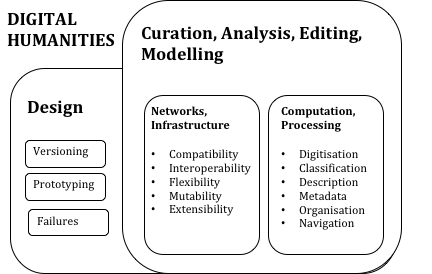
\includegraphics{images/dh01.png}
%   \caption[Digital Humanities]{Digital Humanities model}
% \label{fig:Digital_Humanities}
% \end{figure}

\begin{quotation}
  One of the strongest attributes of the field is that the iterative versioning of digital projects fosters experimentation, risk-taking, redefinition, and sometime failure. [\ldots] It is important that we do not short-circuit this experimental process in the rush to normalize practices, standardize methodologies, and define evaluative metrics.
  \sourceatright{\autocite[p.21]{Burdick2012}}
\end{quotation}

A shortened list of the emerging methods Burdick et al. have identified are shown below \citeyear[p.29-60]{Burdick2012}. A full list can be found in appendix \nameref{app:others}, section~\ref{s:dhmap}\marginnote{§~\ref{s:dhmap}}.

\todo{refer back to this from conclusion or analysis or methodology}

\begin{itemize}
  \item structured mark-up
  \item	natural language processing
  \item	mutability
  \item	digital cultural record
  \item	algorithmic analysis
  \item distant/close, macro/micro, surface/depth
  \item parametrics
  \item	cultural mash-ups
  \item	algorithm design
  \item data visualization
  \item	modelling knowledge
  \item	ambient data
  \item	collaborative authorship
  \item	interdisciplinary teams
  \item	use as performance
  \item narrative structures
  \item	code as text
  \item	software in a cultural context
  \item repurposable content and remix culture
  \item participatory Web
  \item	read/write/rewrite
  \item	meta-medium
  \item	polymorphous browsing
\end{itemize}


% \subsection*{Computer Ethics}

% \begin{quote}
%   One way of characterizing these processes is to use an alliteration that allows us to keep track of some of the core features of RRI in ICT, namely the four “p”s, which are: product, process, purpose and people. The purpose of using the four “p”s is to draw attention to the fact that, in addition to the widely recognized importance of both product and process of technical development, the purpose of the development needs to be considered and people involved in the innovation need to be incorporated in RRI. \autocite{Stahl2013}
% \end{quote}

% \begin{draft}
%   ETHICS\@: PROCESS< PRODUCT< PURPOSE\\
%   ROBOT ETHICS\@: similar to 4-p’s of creativity

%   \autocite{McBride2013}

%   it has three actors: Robot engineer, client and user.

%   4 approaches:\\
%   •	challenge the myth of autonomy\\
%   •	Developing practice-based approaches (in context of it purpose and environment)\\
%   •	Managing ethical variety\\
%   •	A model for human-centred robot ethics

%   Virtuous robot:\\
%   •	Human-centred\\
%   •	Man-machine interdependency\\
%   •	Practice based (context)\\
%   •	Ethical variety
% \end{draft}% chktex 17

\stopcontents[chapters]
